\chapter{Problem definition}
\begin{wrapfigure}{r}{0.5\textwidth}
	\vspace{-60pt}
	\begin{center}
		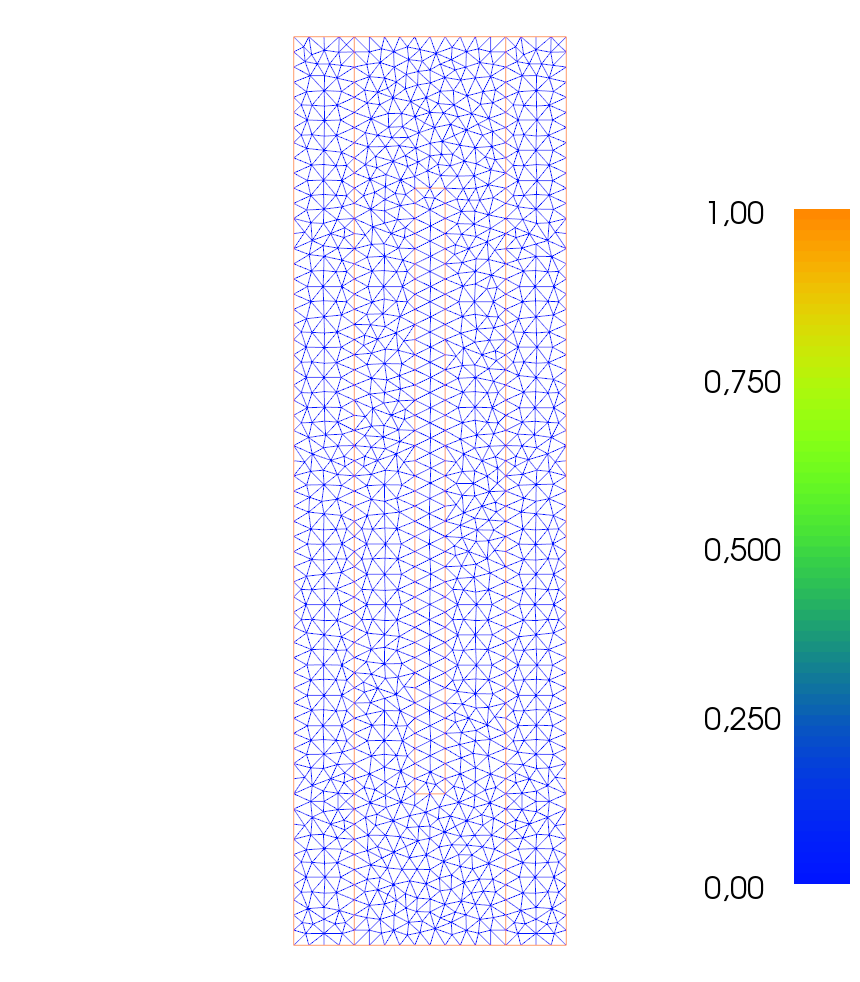
\includegraphics[scale=0.2]{mesh}
	\end{center}
	\vspace{-20pt}
	\caption{Coarse version of the mesh}
	\vspace{-10pt}
\end{wrapfigure}
The model consists of a spinal cord surrounded by space filled with CSF. The cord has a diameter of 10 mm and the fluid space has a diameter of 18 mm. The model also has a inner central spinal canal, 2 mm in diameter. The central spinal canal has height 4 cm and is placed in the center of the mesh which has heigth 6 cm.
\\
\\
\\
\\
\\



\section{Governing equations}



\subsection{Fluid Space}
The fluid in the SAS as well as the central spinal canal is governed by the Navier-Stokes equations
\begin{align}
	\pdi{u_f}{t} + u\cdot \nabla u = -\frac{1}{\rho_f}\nabla p_f + \frac{1}{\rho} \nabla \cdot 		\tau + F&& \text{ in } \Omega_f \label{N-S_m1}
	\\
	\pdi{\rho}{t} +\nabla \cdot(\rho u_f) = 0 && \text{ in } \Omega_f \label{N-S_c1}
\end{align}

where $u_f$ is the fluid velocity, $\rho_f$ is the fluid denisty, $\tau$ is the stress tensor and $F$ are all external volume forces. In addition to the equations (\eqref{N-S_m1}-\eqref{N-S_c1}) comes boundary conditions at the domain boundary. When solving the euqations numerically, manipulation of the coupled equations into simpler equations may lead to problems involving the boundary conditions. Therefore a proper choice of boundary conditions is crucial for stability and existence. 
\\
In this case we will consider incompressible flows, where $\rho$ is constant and $\nabla \cdot u_f = 0$. The stress tensor is given by
\[ \tau_f = -pI + 2 \mu_f \epsilon(u_f) \]
where $\epsilon(u_f) = \frac{1}{2}(\nabla u_f + (\nabla u_f)^T)$
When taking the divergence of the stress tensor the Navier-Stokes equations for incompressible flows take the form

\begin{align}
	\pdi{u_f}{t} + u\cdot \nabla u_f = -\frac{1}{\rho}\nabla p_f + \nu \nabla ^2 u_f + F && 	\text{ in } \Omega_f 
	\\
	\nabla \cdot u_f = 0 && \text{ in } \Omega_f
\end{align}



\subsection{Spinal Cord}
The spinal cord is modeled as a poroelastic medium, which allows for some fluid to flow from the SAS to the central spinal canal. In this case the Biot-equations have been used to include both elasticity and flow in the spinal cord. 
 
\subsection{Weak form}
Equations (3) and (5) will be multiplied by a vector test function, v, and equations (4) and (6) with a scalar test function, q. The equations are then integrated over the entire domain. By using two different test functions the coupled equations can be written as one equation combining the two. \\	
\subsection{Stationary problem, Stokes}
In stokes flow, a steady state pattern have developed for the flow, and convection is neglected. We start with coupling the Stokes flow with a stationary Biot problem. In the CSF the governing equations are
\begin{align}
	- \mu_f \nabla ^2 u_f
	+ \nabla p_f
	= 0 \nonumber \\
	\nabla \cdot u_f = 0
\end{align}
And in the cord
\begin{align}
	- \mu_s \nabla^2 u_s 
	- (\mu_s + \lambda_s) \nabla \nabla \cdot u_s
	+ \nabla p_s = 0 \nonumber \\ 
	- \nabla \cdot \frac{\kappa}{\mu_f} \nabla p_s = 0
\end{align}

Since this is a stationary problem, the first lines of the two equations can be written $-\nabla \cdot \sigma_f = 0$ in $\Omega_f$ and $-\nabla \cdot \sigma_s = 0$ in $\Omega_s$ 




\subsection{Boundary conditions}
We denote the outer wall, $\partial \Omega_f,$, interface $\Gamma$, the top of the cord, $\partial \Omega_{s_t}$, the bottom of the cord $\partial \Omega_{s_b}$, the top of the fluid space $\partial \Omega_{f_t}$ and the bottom of the fluid space $\partial \Omega_{f_b}$. The boundary conditions are as follows: \\
No-slip on the outer walls
\begin{align} u = 0 \text{ on } \partial \Omega_{f_o} \end{align}
Conservation of mumentum at the interface:
\begin{align} \sigma_f \cdot n = \sigma_s \cdot n \text{ on } \Gamma \end{align}
Normal velocity equal at the interface:
\begin{align} u_f \cdot n = - \frac{\kappa}{\mu_f} \nabla p_s \cdot n  \text{ on } \Gamma \end{align}
In the stationary case, the filtration velocity, $-k\nabla p $, corresponds to the total fluid velocity in $\Omega_s$ \\
Prescribed stress on the top and bottom
\begin{align} -\sigma_s \cdot n = p0 \text{ on } \partial \Omega_{f_t} \nonumber \\
			  -\sigma_f \cdot n = p0 \text{ on } \partial \Omega_{s_t} \\
			  -\sigma_s \cdot n = -p0 \text{ on } \partial \Omega_{f_b} \nonumber \\
			  -\sigma_f \cdot n = -p0 \text{ on } \partial \Omega_{s_b} \nonumber
\end{align}



\subsection{Weak form}
Equations (7) and (8) will be multiplied with testFunctions and integrated over their respective domains. The vector equations are multiplied with a vector testFunction, v, and the scalar equations with a scalar testFunction, q. By using two different test functions the coupled equations can be written as one equation combining the two. 
\\
We now integrate the simplified versions of 7-8. Both stress terms and the continuity equation in the Biot problem are integrated by parts. 
\begin{align} (\sigma_f, \nabla v)_{\Omega_f} 
	- (v,\sigma_f \cdot n)_{\partial \Omega_f} 
	= 0 \nonumber \\
	(\nabla \cdot u_f, q)_{\Omega_f} = 0
\end{align}
\begin{align} 
	 (\sigma_s, \nabla v)_{\Omega_s} 
	- (v,\sigma_s \cdot n)_{\partial \Omega_s} 
	= 0 \nonumber \\
	(\frac{\kappa}{\mu_f} \nabla p_s, \nabla q)_{\Omega_s}
	- (q,\frac{\kappa}{\mu_f}\nabla p \cdot n) _{\partial \Omega_s}
	= 0
\end{align}
First of all, using condition (10) we can eliminate the stress terms on the interface, when combining the two equations. Condition (12) can be used to handle the stress term on the top and bottom of the domain. Since we have a no-slip condition on the outer wall, the testFunction v is set to be zero on this boundary so the boundary stress term has now been eliminated from the equations by employing the conditions (10) and (12). 
\\
\\
If we use continuous elements, $u_f = u_s$ on $\Gamma$ by the method itself. For now we settle with this approximation, which might be realistic for low x-velocities and small discplacements. Therefore we can use the condition (11) by rewriting the boundary term in eqn (14). The final form F is:
\begin{align}
	 (\sigma_f, \nabla v)_{\Omega_f} 
	+ (\sigma_s, \nabla v)_{\Omega_s}
	+ (\nabla \cdot u_f, q)_{\Omega_f}
	+ (\frac{\kappa}{\mu_f} \nabla p_s, \nabla q)_{\Omega_s}
	+ (q, u_s \cdot n)_{\partial \Omega_s}
\end{align}
And we seek to solve F = 0. In this case, we assume $u_f = u_s$ on the interface, then (11) is satisfied. At the top and bottom of the cord we also assume $u_s = -\frac{\kappa}{\mu_f}\nabla p_s$(???) 
	
